\documentclass[12pt,a4paper,titlepage]{article}
\usepackage{lab_style}
\usepackage{pdfpages}
\usepackage{eso-pic}
\usepackage{graphicx}
\usepackage{float}
\newcommand\tab[1][1cm]{\hspace*{#1}}

\graphicspath{ {images/} }
  
\begin{document}

\begin{titlepage}
\selectlanguage{english}

%----------------------------------------------------------------------------------------
% TITLE PAGE INFORMATION
%----------------------------------------------------------------------------------------
  \begin{center} % Center everything on the page

  %----------------------------------------------------------------------------------------
  % HEADING SECTIONS
  %----------------------------------------------------------------------------------------
  \textsc{\large Faculty of Computers, Informatics and Microelectronics}\\[0.5cm]
  \textsc{\large Technical University of Moldova}\\[1.2cm] % Name of your university/college
  \vspace{25 mm}

  \textsc{\Large Object-Oriented Modeling and Analysis}\\[0.5cm] % Major heading such as course name
  \textsc{\large Laboratory work \#2}\\[0.5cm] % Minor heading such as course title

\newcommand{\HRule}{\rule{\linewidth}{0.5mm}} % Defines a new command for the horizontal lines, change thickness here

  %----------------------------------------------------------------------------------------
  % TITLE SECTION
  %----------------------------------------------------------------------------------------
  \vspace{10 mm}
  \HRule \\[0.4cm]
  { \LARGE \bfseries Use Case Diagrams. Basic and Alternative Flow. Modeling Languages. }\\[0.4cm] % Title of your document
  \HRule \\[1.5cm]

  %----------------------------------------------------------------------------------------
  % AUTHOR SECTION
  %----------------------------------------------------------------------------------------
      \vspace{30mm}

      \begin{minipage}{0.4\textwidth}
      \begin{flushleft} \large
      \emph{Author:}\\
      Cernei \textsc{Liviu}
      \end{flushleft}
      \end{minipage}
      ~
      \begin{minipage}{0.4\textwidth}
      \begin{flushright} \large
      \emph{Supervisor:} \\
      Mihail \textsc{Gavrilița} % Supervisor's Name
      \end{flushright}
      \end{minipage}\\[4cm]

      \vspace{5 mm}
      % If you don't want a supervisor, uncomment the two lines below and remove the section above
      %\Large \emph{Author:}\\
      %John \textsc{Smith}\\[3cm] % Your name

      %----------------------------------------------------------------------------------------
      % DATE SECTION
      %----------------------------------------------------------------------------------------

      {\large Chișinau 2018}\\[3cm] % Date, change the \today to a set date if you want to be precise

      %----------------------------------------------------------------------------------------
      % LOGO SECTION
      %----------------------------------------------------------------------------------------

      %\includegraphics{red}\\[0.5cm] % Include a department/university logo - this will require the graphicx package

      %----------------------------------------------------------------------------------------

      \vfill % Fill the rest of the page with whitespace
      \end{center}
      
\end{titlepage}

\cleardoublepage

\newpage

\pagenumbering{arabic}
\setcounter{page}{1}
\setcounter{secnumdepth}{4}

\addtocontents{toc}{\protect\thispagestyle{empty}} % no page number on the table of contents page
\cleardoublepage


\phantomsection
\addcontentsline{toc}{section}{Introduction}
\section*{Laboratory work \#2}
\phantomsection

\section{Tasks}
\begin{itemize}
	\item
	Model your application using 3 Use Case Diagrams;
	\item 
	Create the basic and alternate flows of 3 most important use cases.
\end{itemize}

\section{Theory}
Use case diagrams are used to describe a set of actions (use cases) that some system (subject) can perform in collaboration with one or more external users of the system (actors).

\subsection{Use case diagram elements}
\begin{enumerate}  
	\item Actor - Someone who interacts with use case (system function).
	\item Use Case - System function (process - automated or manual)
	\item Communication Link - a solid link which shows the participation of an actor in a use case 
\end{enumerate}


\subsection{Use Case Relationship}
\begin{enumerate}  

	\item Include
	\begin{enumerate}
		\item When a use case is using functionality of another use case.
		\item An include relationship is depicted with a directed arrow having a dotted line. 
		\item The stereotype "include" identifies the relationship as an include relationship.
	\end{enumerate}
	\item Extends
	\begin{enumerate}  
		\item Whem a use case can be divided in another use cases.
		\item Depicted with a directed arrow having a dotted line. 
		\item The stereotype "extends" identifies as an extend relationship
	\end{enumerate}
	\item Generalization
	\begin{enumerate}  
		\item A generalization relationship is a parent-child relationship between use cases.
		\item The child use case in the generalization relationship can replace the parent use case.
		\item Generalization is shown as a directed arrow with a triangle arrowhead.
	\end{enumerate}
\end{enumerate}

\section{Use Case Diagrams}
In Figure ~\ref{fig:student} is represented the Use Case diagram for the actor "student".
\begin{figure}[H]
\centering
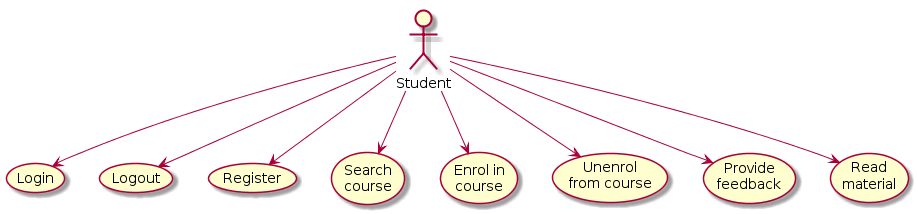
\includegraphics[width=\textwidth]{student}
\caption{Student Use Case diagram}
\label{fig:student}
\end{figure}

In order to be able to login the student should have an account. Also, to logout the student should firstly login. Another case is the registration - the student must provide personal information (first / last name, year of study, university, faculty. group etc.). After registration, the user searches a course, the student can input the name of teacher or the title of the lecture.\par
Enrolment in a course is performed by selecting a course, clicking the [Enrol] button and accepting the confirmation message. The same with the unenrollment procedure.
Finally, the student selects a course in which he is already enroled and can start reading the content.
At the bottom of the page the student also can find the "Feedback" form.

In Figure ~\ref{fig:teacher} is represented the Use Case diagram for the actor "teacher".
\begin{figure}[H]
\centering
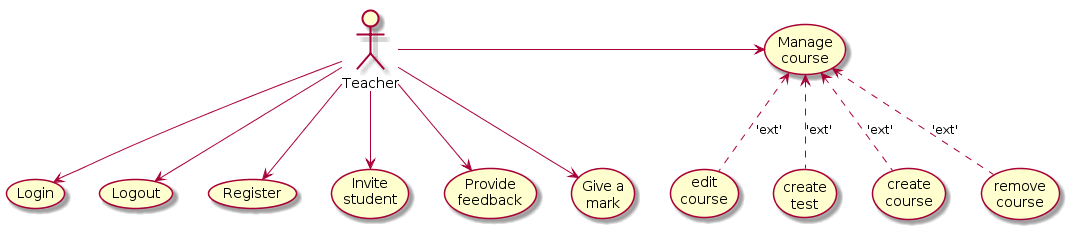
\includegraphics[width=\textwidth]{teacher}
\caption{Teacher Use Case diagram}
\label{fig:teacher}
\end{figure}
The teacher has access like the student user, but with additional privileges. He invite a student to one of his own courses. The teacher is responsible for giving marks or evaluating the student at the end of course.\par
Also, the techer is in control of the content of the course - we can say that he can perform "CRUD" operations on his own courses.

In Figure ~\ref{fig:admin} is represented the Use Case diagram for the actor "administrator".
\begin{figure}[H]
\centering
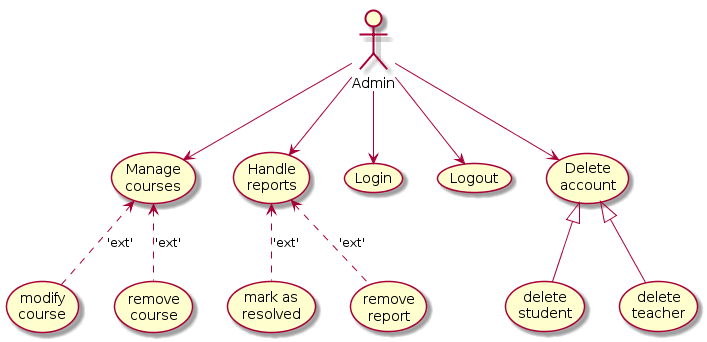
\includegraphics[width=\textwidth]{admin}
\caption{Admin Use Case diagram}
\label{fig:admin}
\end{figure}

The administrator can do almost everything he wants. He can manage courses from any teacher, can remove any accounts. Also he is responsible for handling reports.

\section{Flow of Events}
\begin{itemize}
\item
\noindent\textbf{Student Use Case diagram - Enrol in course}
\begin{description}
    \item[Success scenario:]
\end{description}
\renewcommand{\labelenumii}{\arabic{enumii}}
\begin{itemize}
  \item 1. The student navigates to "Courses" page
  \item 2. The student selects from the list a course
  \item 3. The student clicks the [Enrol] button.
  \item 4. The system outputs success message.
\end{itemize}
\begin{description}
    \item[Alternate flow:]
\end{description}
\begin{itemize}
  \item 1.a The student enroled to the course by a teacher, other steps are not performed.
  \item 2.a The student inputs name of course in the search box
\end{itemize}

\item
\noindent\textbf{Teacher Use Case diagram - Create course}
\begin{description}
    \item[Success scenario:]
\end{description}
\renewcommand{\labelenumii}{\arabic{enumii}}
\begin{itemize}
  \item 1. The teacher navigates to "Courses" page
  \item 2. The teacher clicks the [New] button.
  \item 3. The teacher writes the title, date, content.
  \item 4. The teacher clicks the [Save] button.
  \item 5. The system outputs success message.
\end{itemize}
\begin{description}
    \item[Alternate flow:]
\end{description}
\begin{itemize}
  \item 3.a The teacher writes the title, date and imports the pdf file with the content.
\end{itemize}

\item
\noindent\textbf{Admin Use Case diagram - Login}
\begin{description}
    \item[Success scenario:]
\end{description}
\renewcommand{\labelenumii}{\arabic{enumii}}
\begin{itemize}
  \item 1. The admin navigates to "Login" page
  \item 2. The admin inputs correct username and correct password.
  \item 3. The admin clicks the [Login] button.
  \item 4. The system outputs success message.
\end{itemize}
\begin{description}
    \item[Alternate flow:]
\end{description}
\begin{itemize}
  \item 2.a The admin inputs wrong username or wrong password, fails to login but attempts one more time with correct username and correct password.
  \item 3.a The admin presses the [Enter] key on the keyboard.

\end{itemize}
\end{itemize}

\clearpage
\cleardoublepage

\end{document}
